\documentclass[a4paper,12pt]{article} 
\usepackage[T2A]{fontenc}			
\usepackage[utf8]{inputenc}			
\usepackage[english,russian]{babel}	
\usepackage{amsmath,amsfonts,amssymb,amsthm,mathtools} 
\usepackage[colorlinks, linkcolor = blue]{hyperref}
\usepackage{upgreek}\usepackage[left=2cm,right=2cm,top=2cm,bottom=3cm,bindingoffset=0cm]{geometry}
\usepackage{multirow}
\usepackage{graphicx,wrapfig,lipsum}
\usepackage{xcolor}
\usepackage{pgfplots}
\usepackage{setspace}


\begin{document}

\title{
3.2.8.

Релаксационные колебания.
\author{Семёнов Андрей Б02-010}
}
\date{22 сентября 2021г.}

\maketitle

\newpage

\textbf{Цель работы:} Изучение ВАХ нормального тлеющего разряда; исследование релаксационного генератора на стабилитроне.

\textbf{В работе используются:} стабилитрон СГ-2 (газонаполненный диод) на монтажной панели, магазин ёмкостей, магазин сопротивлений, источник питания, амперметр, вольтметр, осциллограф.

\section{Теоретические сведения.}

\begin{wrapfigure}[22]{r}{0.5\textwidth}
   		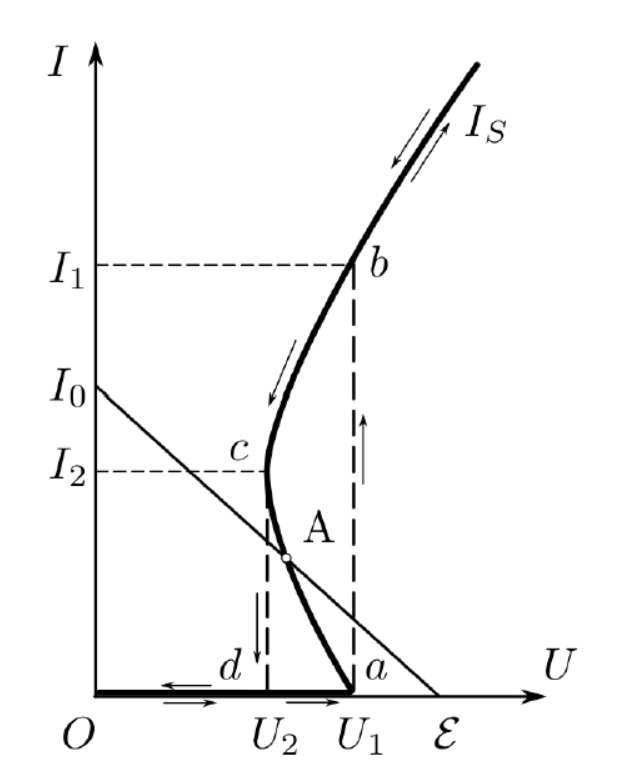
\includegraphics[width=0.4\textwidth]{plot}
    	\caption{Зависимость тока от напряжения для газоразрядной лампы }
    	\label{ris:plot}
\end{wrapfigure}
	
	
	%\begin{flushleft}
		%\begin{spacing}{1.6}
		
В работе исследуются релаксационные колебания, возбуждаемые в электрическом контуре, состоящем из ёмкости $C$, резистора $R$ и газоразрядного диода c $S$-образной вольт-амперной характеристикой. 
\\
\textit{Автоколебания} — незатухающие колебания в диссипативной динамической системе с 
нелинейной обратной связью, поддерживающиеся за счёт энергии постоянного, то есть непериодического внешнего воздействия. 
\\
В апериодической системе, в которой за период автоколебаний теряется вся накопленная энергия, автоколебания становятся \textit{релаксационными} и могут по форме очень сильно отличаться от колебаний синусоидальных. 
\\
Автоколебательная система, не содержащая одного из накопителей колебательной энергии (например, индуктивности или емкости), называется \textit{вырожденной}. Колебания в такой системе могут быть только релаксационными. 
\\
На рисунке (\ref{fig:plot}) представлена принципиальная схема вольт-амперной характеристики исследуемой газоразрядной лампы. 
Зависимость тока от напряжения для газоразрядной лампы не подчинятся закону Ома и характеризуется рядом особенностей, представленных на рисунке (\ref{fig:plot}) вместе с нагрузочной прямой $I=I_{0}\cdot(1 - U/\varepsilon)$
\begin{figure}[h]
\center{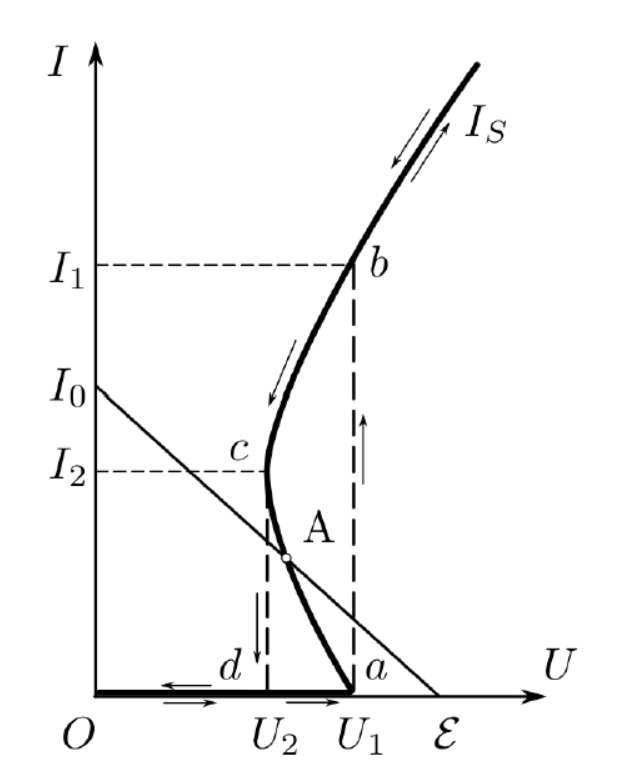
\includegraphics[scale=0.5]{plot.png}}
\caption{ВАХ стабилитрона}
\label{fig:plot}
\end{figure}
Найдем, когда автоколебания возможны: 
$$
\frac{dW}{dt} = -P(t)
$$
где:
$W$ -- энергия, запасенная в колебательном контуре;
$P(t)$ -- мощность потерь.
Интергируя по периоду колебаний $T$:
$$
W = W_0 - \int\limits_0^T P(t)dt 
$$
Если $P(t)$ знакопеременна, то можно обеспечить энергетический баланс $\int\limits_0^T P(t)dt = 0$ и, следовательно, возбудить автоколебания. Для выполнения таких условий необходимо наличие элемента цепи с отрицательным дифференциальным сопротивлением:
$$
R_{diff} = \frac{dU}{dI} < 0
$$
Таким <<сопротивлением>> обладают системы на <<падающих>> участках вольт-амперных характеристик, например наша газоразрядная лампа.
\subsection*{Рассмотрим экспериментальную установку} 
\begin{figure}[h]
\center{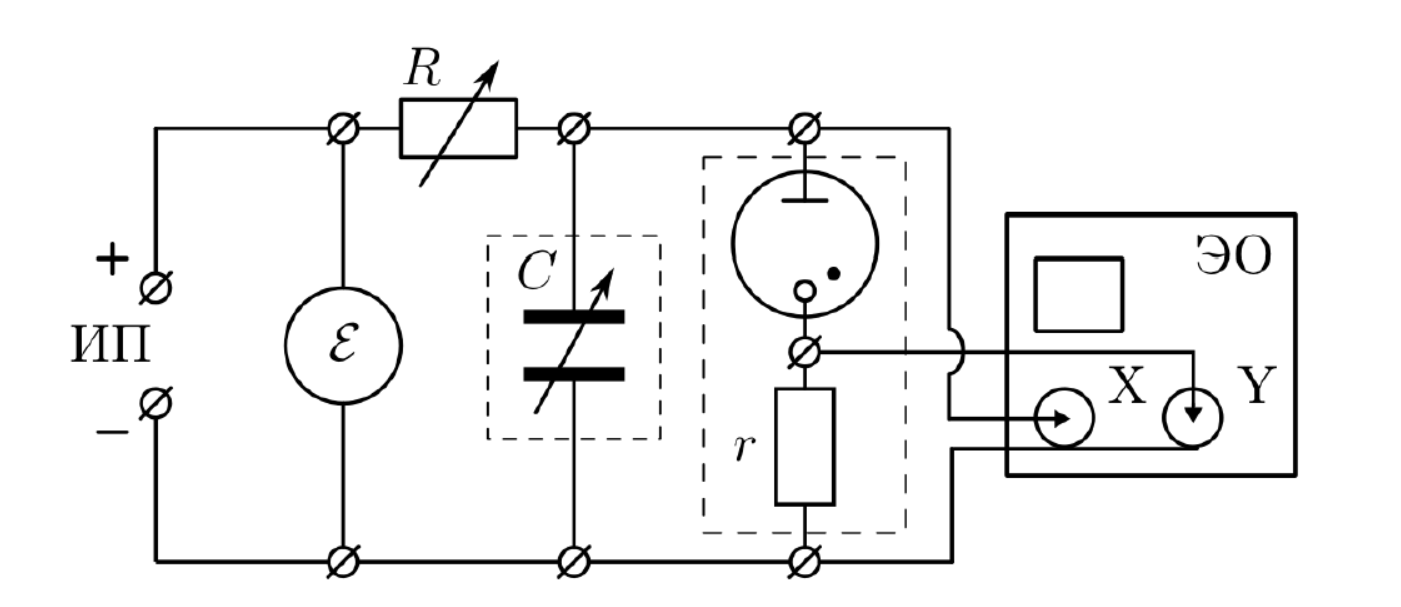
\includegraphics[scale=0.5]{fac1.png}}
\caption{Схема установки для исследования релаксационных колебаний}
\label{fig:fac1}
\end{figure}
Выясним, при каком условии в данном случае колебательный процесс возможен...
В стационарном режиме $dU/dt = 0$, а ток через лампу:
$$
I = \frac{\varepsilon - U}{R + r}
$$
Это происходит тогда, когда нагрузочная прямая пересекает <<падающий>> участок ВАХ-а стабилитрона, где $I'_S(U) < 0$. Если при этом выполняется условие
$$
R + r < -\frac{1}{I'_S(U_A)}
$$
Опишем колебательный процесс:
\begin{enumerate}
\item Отсчитываем время с момента, когда $U_C = U_2$.
\item При зарядке конденсатора через сопротивление $R$ напряжение на нем увеличивается.
\item Как только оно достигает напряжения зажигания $U_1$, лампа начинает проводить ток, причем прохождение тока сопровождается разядкой конденсатора. В самом деле, батарея $\varepsilon$, подключенная через $R$ не может поддерживать необходимую для горения лампы величину тока.
\item Во время горения лампы конденсатор разряжается, и когда напряжение на нем достигает потенциала гашения $U_2$, лампа перестает проводить ток, а конденсатор вновь начинает заряжаться.
\item Возникают релаксационные колебания с амплитудой $U_1 - U_2$.
\end{enumerate}
\begin{figure}[h]
\center{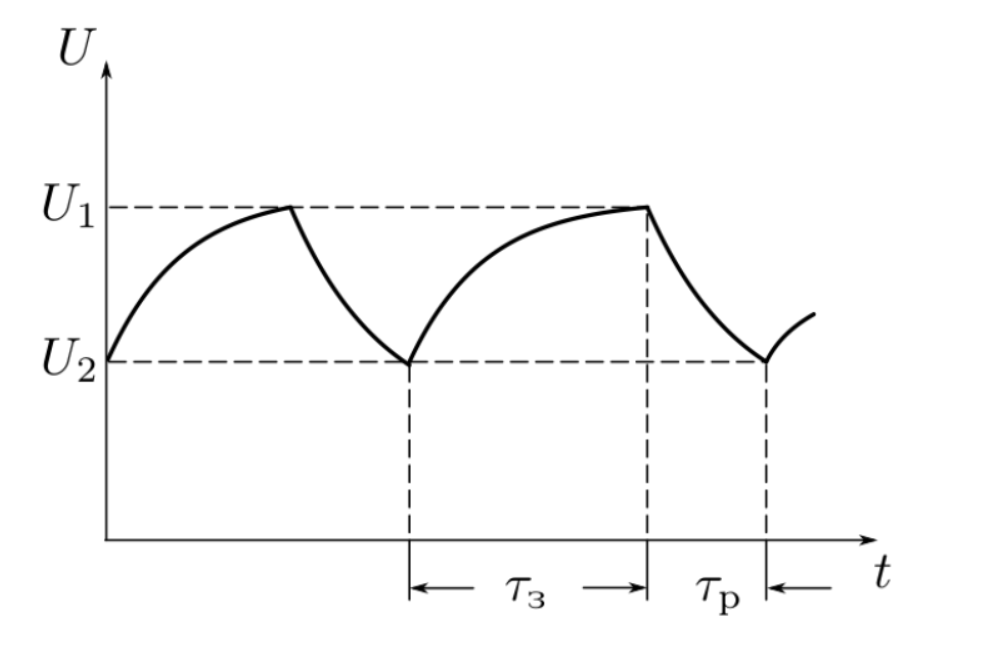
\includegraphics[scale=1]{oscillogramm.png}}
\caption{Осциллограмма релаксационных колебаний}
\label{fig:oscillogramm}
\end{figure}
Расчитаем период колебаний: поскольку $R$ сильно больше сопротивления заряженной лампы, то $\tau_3 >> \tau_p$
$$
T = \tau_3 + \tau_p \approx \tau_3
$$
Во время зарядки конденсатора лампа не горит ($I(U) = 0$), имеем
$$
RC\frac{dU}{dt} = \varepsilon - U
$$
Решая это уравнение:
$$
U = \varepsilon - (\varepsilon - U_2)\exp(\frac{-t}{RC})
$$
В момент зажигания $t = \tau_3$, $U = U_1$, поэтому
$$
U_1 = \varepsilon - (\varepsilon - U_2)\exp(\frac{-\tau_3}{RC})
$$
Теперь нетрудно найти период колеаний:
$$
T \approx \tau_3 = RC\ln\frac{\varepsilon - U_2}{\varepsilon - U_1}
$$
\section{Выоплнение работы}
\subsection*{Характеристика стабилитрона}
$r = 5.4$ кОм
\\
Произведем измерения ВАХ-ки стабилитрона с сопротивлением $r$ при возрастании и убывании напряжения $U$ и выясним потенциалы гаешения и зажигания $U_1$ и $U_2$, а также соответствующие им токи $I_1$ и $I_2$.
\begin{table}[h]
\centering
\begin{tabular}{|l|l|l|l|}
\hline
$U$, V & $I_{up}$, mA  & $U$, V & $I_{down}$, mA      \\ \hline
75.33  & 0.007  & 133.45  & 11.017   \\ \hline
79.95  & 0.008  & 124.69   & 9.294   \\ \hline
84.53 & 0.008  & 113.32  & 7.383   \\ \hline
88.87  & 0.009  & 103.01 & 5.571    \\ \hline
91.52  & 0.009  & 94.02  & 3.903   \\ \hline
96.97  & 0.01  &90.62   & 3.2   \\ \hline
98.43  & 0.01  & 88.2  & 2.803   \\ \hline
99.55  & 0.01  & 87  & 2.582   \\ \hline
99.81  & 4.893  & 85.54  & 2.305   \\ \hline
104.24  & 5.731  & 84.16  & 2.066   \\ \hline
114.08  & 7.511  & 82.21  & 1.691   \\ \hline
123.36  & 9.167  & 79.54  & 1.176   \\ \hline
133.82  & 11.068  & 79.26  & 0   \\ \hline
144.23  & 12.786  & 75.22  & 0   \\ \hline
\end{tabular}
\end{table}
Теперь построим графики по этим значениям:
\begin{figure}[h]
\center{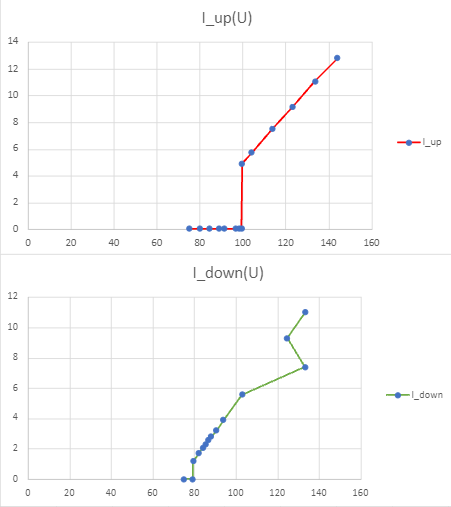
\includegraphics[scale=1]{relation1.png}}
\caption{ВАХ стабилитрона при поднятии и опускании напряжения}
\label{fig:relation1}
\end{figure}
Таким образом, потенциалы и токи зажигания и гашения: 
$U_1 = 98.6 V$\\
$U_2 = 77.6 V$\\
$I_1 = 4.9 mA$\\
$I_2 = 1.3 mA$\\
\subsection*{Осциллограммы релаксационных колебаний}
Установим $C = 50$ нФ и $R = 900$ кОм. Выставим s = 118.1 В. 
Оценим соотношении времен зарядки и разрядки. Для этого определим по осциллографу: 
$\tau_3 = 42$мс
$\tau_p = 0.5$мс
Видим, что раздичия существенны, начит все нормально и можем вычислить частоту:
$$
\nu = \frac{1}{T} \approx \frac{1}{\tau_3} = 24 Hz
$$
Определим критическое сопротивление, при котором пропадают колебания:
$$
R_{crit} = 144 kOhm
$$
Далее фиксируем $R$ и определяем $\varepsilon$ критическое, когда $R$ не слишком превышает(???) $R_{crit}$:
$$
\varepsilon_{crit} = 152 V
$$
Теперь $T(C)$, при изменении $C$ от 2 до 50 нФ и постоянном $\varepsilon$:
\begin{table}[h]
\centering
\begin{tabular}{|l|l|}
\hline
$C$, nF & $T$, ms     \\ \hline
 2 &   1.2  \\ \hline
 5 &  1.2   \\ \hline
 6 &  1.3   \\ \hline
 7 &  1.5   \\ \hline
 8 &   1.8  \\ \hline
 9 &   2.1  \\ \hline
 10 &  2.5   \\ \hline
 15 &  4.5   \\ \hline
 20 &   6.8  \\ \hline
 25 &  8.6   \\ \hline
 30 &  11.1   \\ \hline
 35 &   12.6  \\ \hline
 40 &   13.9  \\ \hline
 45 &    14.9 \\ \hline
 50 &    16.8 \\ \hline
\end{tabular}
\end{table}
\begin{figure}[h]
\center{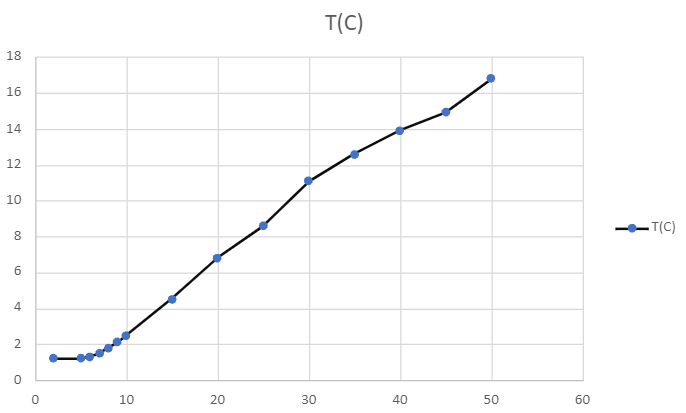
\includegraphics[scale=1]{relation2.png}}
\caption{Зависимость $T(C)$}
\label{fig:relation2}
\end{figure}
Далее зависимость $T(R)$:
\begin{table}[h]
\centering
\begin{tabular}{|l|l|}
\hline
$R$, kOhm & $T$, ms     \\ \hline
 200 &   9.3  \\ \hline
 300 &  12.7   \\ \hline
 400 &  13.6  \\ \hline
 500 &  22   \\ \hline
 600 &   33  \\ \hline
 700 &   37  \\ \hline
 800 &  40   \\ \hline
 900 &  44   \\ \hline
 1000 &   49  \\ \hline
\end{tabular}
\end{table}
\begin{figure}[h]
\center{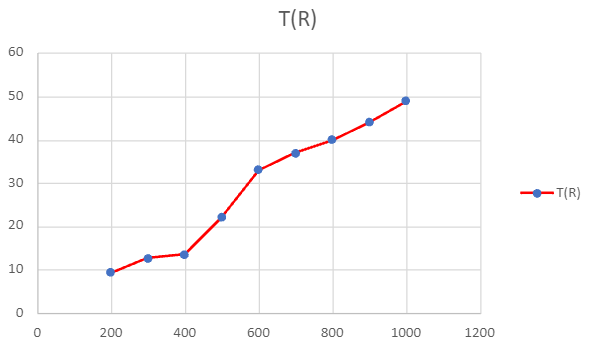
\includegraphics[scale=1]{relation3.png}}
\caption{Зависимость $T(R)$}
\label{fig:relation3}
\end{figure}
\subsection*{Фазовые траектории релаксационных колебаний}
\begin{figure}[h]
\center{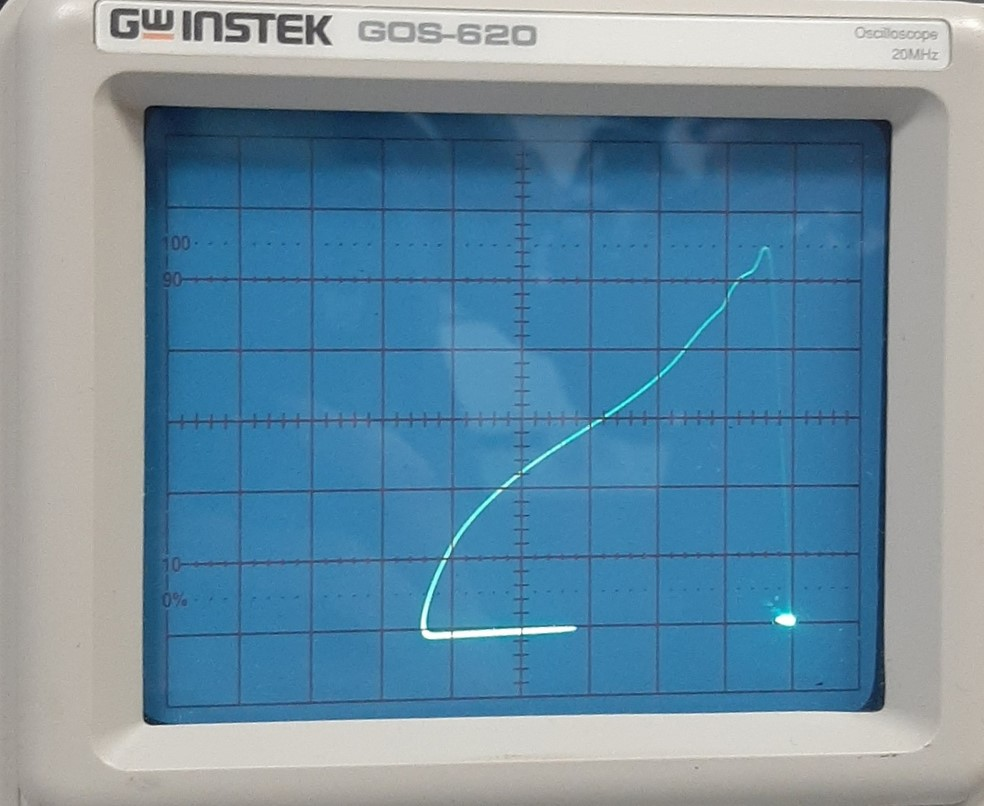
\includegraphics[scale=1]{phtrajectory.jpg}}
\caption{Фазовая траектория}
\label{fig:phtrajectory3}
\end{figure}
\newpage
\end{document}